\begin{chapter}{\label{cha:afm}Simulating the surface of a ``Floppy Wire''}
\section{\label{section:sfwire} Superfluid wire experiments}
Developments in flow visualization at very low temperatures
\cite{Guo2014,Fisher2014} have
driven recent progress in the turbulence in superfluid $^4$He and
$^3$He-B. Experiments and theory have highlighted effects
such the existence of classical and
nonclassical turbulent regimes \cite{WalmsleyGolov2008}, and
energy transfer over length scales, both
direct \cite{Barenghi2014} and inverse
\cite{WalmsleyTompsett2013,Baggaley2014}.
At the same time, improvements in the generation, observation and control of quantum
vortices in atomic Bose--Einstein condensates\cite{Henn2009,Freilich2010,Aioi2011,Neely2013,Kwon2014}
has added a character of interdisclinarity to the study of
turbulence in quantum fluids.

In many superfluid helium experiments \cite{VinenSkrbek2008}, turbulence
is generated by moving grids \cite{Davis2000},
wires \cite{Guenault1986,Bradley2005,Bradley2011,Fisher2001,Goto2008},
forks \cite{Blaauwgeers2007,Bradley2012} or spheres \cite{Schoepe1995}.
Although macroscopically polished, the surface of these objects is
rough on the length scale of the superfluid vortex core, which is of
the order of $10^{-10}~\rm m$ in $^4$He
and $10^{-8}~\rm m$ in $^3$He.  As an example, Fig.~\ref{fig:afmimg}(a) is an atomic force microscope (AFM) image showing the microscopic detail on the surface of a  single--core NbTi `floppy' wire used for generating superfluid turbulence  \cite{Bradley2011}.  Note the appearance of an elongated scratch, typical of such wires.  No direct flow visualization is available on these microscopic length scales and, as such, 
superflow in the presence of walls remains poorly understood. In principle, the superfluid boundary conditions should
be straighforward.
In the simplest case of a boundary at rest, the superfluid velocity
component which is perpendicular to the boundary must be equal to
zero at the boundary, while the tangential component can slip.
In practice, nucleation of quantum vorticity complicates
this idealized Eulerian picture.

\begin{figure}[t]
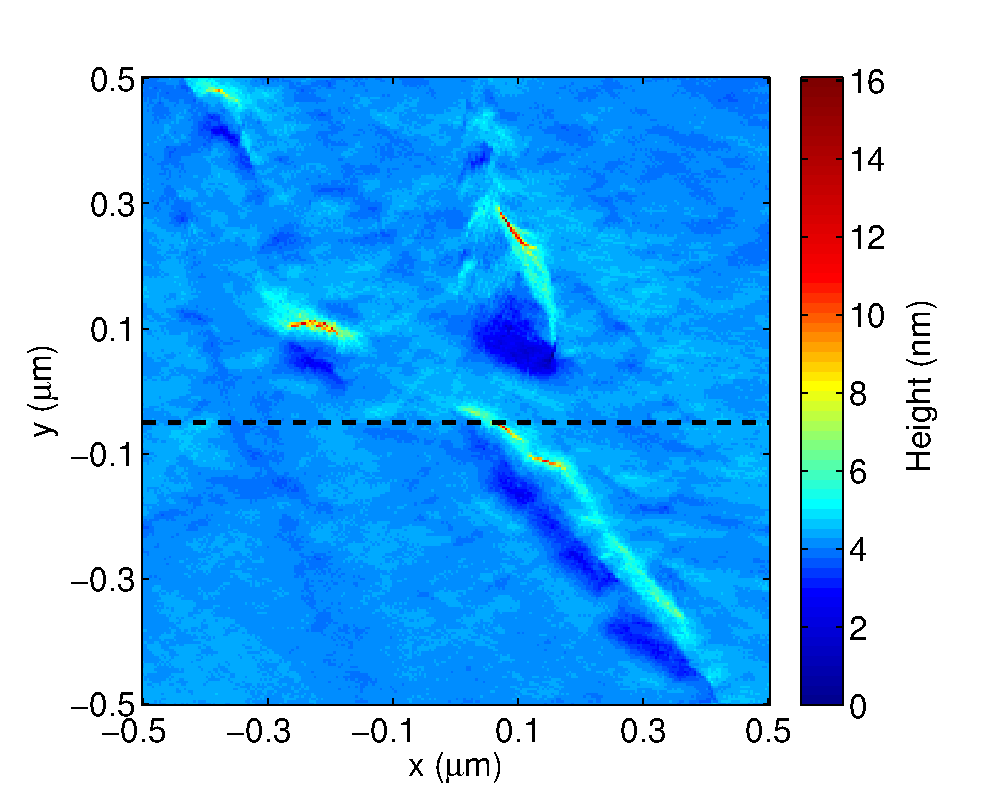
\includegraphics[width=0.45\linewidth]{./afm/figures/afm}
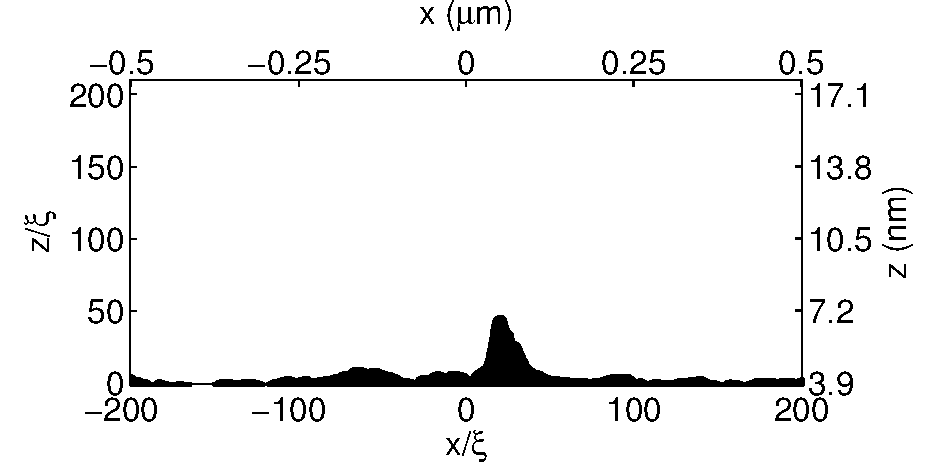
\includegraphics[width=0.45\linewidth]{./afm/figures/xz-vs-mmnm}
\caption{\label{fig:afmimg} (a) AFM image of a typical NbTi wire used for the generation of quantum turbulence.  The roughness of the surface is seen in the form of scratches along the surface. (b)  The cross-section of the AFM data along $y = -0.05 \mu$m (indicated by the dashed line in (a)) is imposed as a surface in our 2D simulations.}  
%The scaling ($\alpha=30$) between real and dimentionless units is evident from the dual axes.}
\end{figure}
The established theoretical approaches used to successfully describe
homogeneous superfluid turbulence away from boundaries can falter in the presence of realistic boundaries.
First consider the vortex filament method of Schwarz
\cite{Schwarz,Hanninen-PNAS}. Its application to relatively simple and smooth
boundaries, such as spheres \cite{Hanninen-sphere,Kivotides-sphere} and
hemispheres \cite{Schwarz-bump}, has proved
cumbersome due to the complex system of images which is required.
Its starting assumption, that the vortex core
is infinitesimally smaller than any other length scale, makes it
unsuitable for realistic boundaries of roughness comparable to
the vortex core size.  Moreover Schwarz's approach requires arbitrarily seeding
vortex loops, because it does not account for vortex nucleation.
Another approach which suffers similar difficulties \cite{Henderson} is
the two--fluid Hall--Vinen--Bekarevich--Khalatnikov (HVBK)
equations \cite{Salort2011,Salort2012}. Moreover, the HVBK equations are coarse--grained over
length scales larger than the average vortex separation, hence the
boundary conditions require further assumptions or the introduction of
unknown sliding/pinning parameters.

A practical dynamical model of superflow near boundaries of arbitrary
shape which is powerful enough to describe vortex nucleation is
the Gross--Pitaevskii equation (GPE) \cite{RobertsBerloff}.  While the GPE is an accurate quantitative description of atomic condensates, it provides only a qualitative model of superfluid helium.  Frisch {\it et al.} pioneered the GPE approach by simulating superflow past a cylinder, observing vortex pair nucleation above a critical flow speed \cite{Frisch1992}.  Subsequent GPE-based works have further elucidated vortex generation past a cylinder \cite{Cylinder}, as well as spheres and half-spheres \cite{Sphere}, and elliptical objects \cite{Ellipse}.    Nevertheless, at this stage of investigation, the GPE is the optimum tool 
to gain physical insight into the flow of a superfluid over
rough surfaces typical of experiments.
\section{\label{section:afmimage} The ``Floppy Wire'' AFM image}
\section{\label{section:gpeafm} GPE with AFM surface}
\section{\label{section:2dafm} 2D clusters and backflow vortex generation}
\section{Theoretical Model}
Within the GPE model the condensate is parameterized via a macroscopic wavefunction $\Psi({\bf r},{t})$; this specifies the condensate (number) density $n({\bf r},{t})=|\Psi({\bf r},{t})|^2$.  The GPE is
\begin{equation}
i \hbar \frac{\partial\Psi}{\partial t} 
= \left(-\frac{\hbar^2}{2m}\nabla^2 + V + g|\Psi|^2 + i \hbar v \frac{\partial \Psi}{\partial x} - \mu \right) \Psi.
\label{eq:gpe1}
\end{equation}
\noindent
% $g=4 \pi \hbar^2 a_{\rm s}/m$
where $m$ is the mass of one atom, $g$ is a coefficient that characterizes the atomic interactions, and $\mu$ is the chemical potential (energy
per atom).  $V({\bf r},t)$ is the external potential acting on the condensate; we will take this to represent the rough surface (see below).  The speed-dependent term provides a Galilean transformation to a reference frame moving with speed $v$ along $x$; this will enable us to model flow past the surface.

We express density in terms of the density at infinity $n_0$, energy in terms of $\mu$, length in terms of the healing length $\xi=\hbar/\sqrt{m n_0 g}$, and speed in terms of the sound speed $c=\sqrt{n_0 g/m}$; our unit of time follows as $\tau=\xi/c$.  In practice we solve the corresponding dimensionless GPE $i(\partial\Psi'/\partial t') = \left[-(1/2)\nabla^2 + V' + |\Psi'|^2 + iv (\partial \psi/\partial x)- 1 \right] \Psi'$, where the prime indicates dimensionless quantities.

The AFM data depicted in Fig. \ref{fig:afmimg}(a) provides a two-dimensional map of the height of the surface, $z=h(x,y)$.  We convert the $z$-scale into units of healing length using the value for $^{4}$He, $\xi_{4}=0.66 \AA$\footnote{The vortex rings experiments of Rayfield \& Reif \cite{Rayfield1964} 
suggests a $^4$He vortex core radius of around $a_0=1\AA$. We define the vortex 
core in our simulations as the radius at which the density drops to 
50\% of the value at infinity, so $a_0 = 1.52\xi$. This gives us a
$\xi=1\AA/1.52 \approx 0.66\AA$ for $^4$He.}.  Due to the lack of resolution in the $x$ and $y$ directions it is not possible to convert these on the scale of $\xi_{4}$; instead these directions are given arbitrary conversions into healing lengths with the range $-0.5 \mu$m $\leq x,y \leq 0.5 \mu$m taken to be $-200 \xi \leq x,y \leq 200 \xi$, as shown in Fig. \ref{fig:afmimg}.
%To impose a boundary the AFM image data is first scaled into dimentionless units, $h(x,y)$. 
To model the boundary through the external potential $V(x,y,z)$, we set $V=0$ everywhere apart from below the surface, where we set $V=50 \mu$; this value is sufficiently large that it effectively contrains the density to zero.  

Our numerical approach is to first obtain the stationary solution for the static fluid $(v=0)$, achieved via imaginary time propagation of the GPE \cite{Minguzzi2004}.  From this initial condition the GPE is then propagated in real time, with the fluid speed $v$ ramped up smoothly from zero up to its required value.  

To assess the role of tall prominences in the surface, we will also consider cases where the surface height $z=h(x,y)$ is truncated to a percentage $\beta$ of the maximum height $h_0$, i.e. $h(x,y) \rightarrow h(x,y) H(z/h_0=\beta)$, where $H(z)$ is the Heaviside step function ($\beta=100\%$ corresponds to no truncation, $\beta=0$ corresponds to complete truncation).

%at a height $z_t$, i.e. 

%Accordingly we define the external potential to be,
%\begin{equation}
%V(x,y,z) =
%\begin{cases}
%50 \mu &\mbox{if } z < [h(\alpha x,\alpha y)-z_0]H(z_t-z)  \\
%0 &\mbox{if } z > [h(\alpha x,\alpha y)-z_0]H(z_t-z).
%\end{cases}
%\label{eq:potential2D}
%\end{equation}
%where H(z) is the Heaviside step function, $z_t$ is a truncation level, $z_0$ is a shift in height, 
%and $\alpha$ is a scaling factor. Truncating and scaling $h(x,y)$ acts as a crude way of varying 
%the roughness of simulated boundaries. Finally, linear interpolation is applied so 
%that $V(x,y,z)$ is continuous in $x$ and $y$.


%We take the external potential acting on the condensate $\widetilde{V}=\widetilde{V}(\tilde{x},\tilde{y},\tilde{z})$ to represent the boundary of the surface depicted in Fig. \ref{fig:afmimg} (details below).

%We cast the GPE in the following
%dimensionless form
%\begin{equation}
%i \frac{\partial\psi}{\partial t} = \left(-\frac{1}{2}\nabla^2 + V + |\psi|^2 - 1 \right) \psi.
%\label{eq:gpe2}
%\end{equation}
%\noindent
%using the healing length $\xi = \hbar/\sqrt{m n_0 g}$ as unit of distance, where $n_0$ is the density of the uniform condensate, $(\xi/c)$ as unit of time, where $c=\sqrt{n_0 g/m}$ is the speed of sound and $\sqrt{n_0}$ as the wavefunction unit. 

%To mimic flow past the surface, we transform the GPE to a reference frame moving with speed $v$ in the positive $x$ direction via the addition of the Galilean term $ iv \partial \psi/\partial x$ to the right-hand side of Eq.~\ref{eq:gpe2}.

In 2D, we solve the (dimensionless) GPE using the 4th-order Runge--Kutta
method, with periodic boundary conditions, on a $1024\times512$
grid with uniform spacing $\Delta=0.4$. %along $x$ and $z$ directions, corresponding to the computational region $-204.8 \leq x/\xi \leq 204.8$, $-102.4 \leq z/\xi \leq 102.4$. In 3D the entire AFM image can be modeled. In 2D $y$ is fixed so that the slice 
$y = -0.05~\mu$m is used. 



%Due to the lack of resolution in the $xy$ plane in comparison to $z$ a scaling factor of $\alpha=30$ is employed.We choose $z_0$ so that the minimum of $h(x,y)=0$. The 2D scaling between real and dimentionless units can be seen in Figure \ref{fig:afmimg}.

\subsection{Typical Evolution}

\begin{figure*}
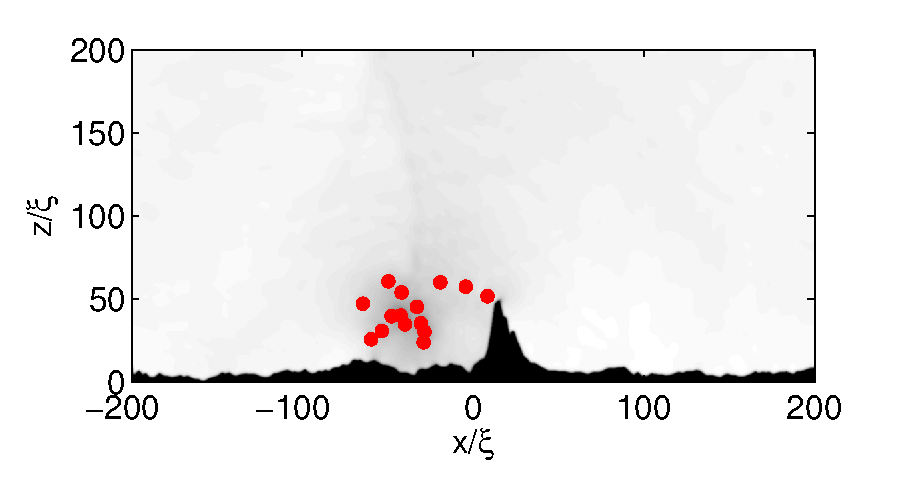
\includegraphics[width=0.35\linewidth]{./afm/figures/prog-35-500}\hspace{-0.6cm}
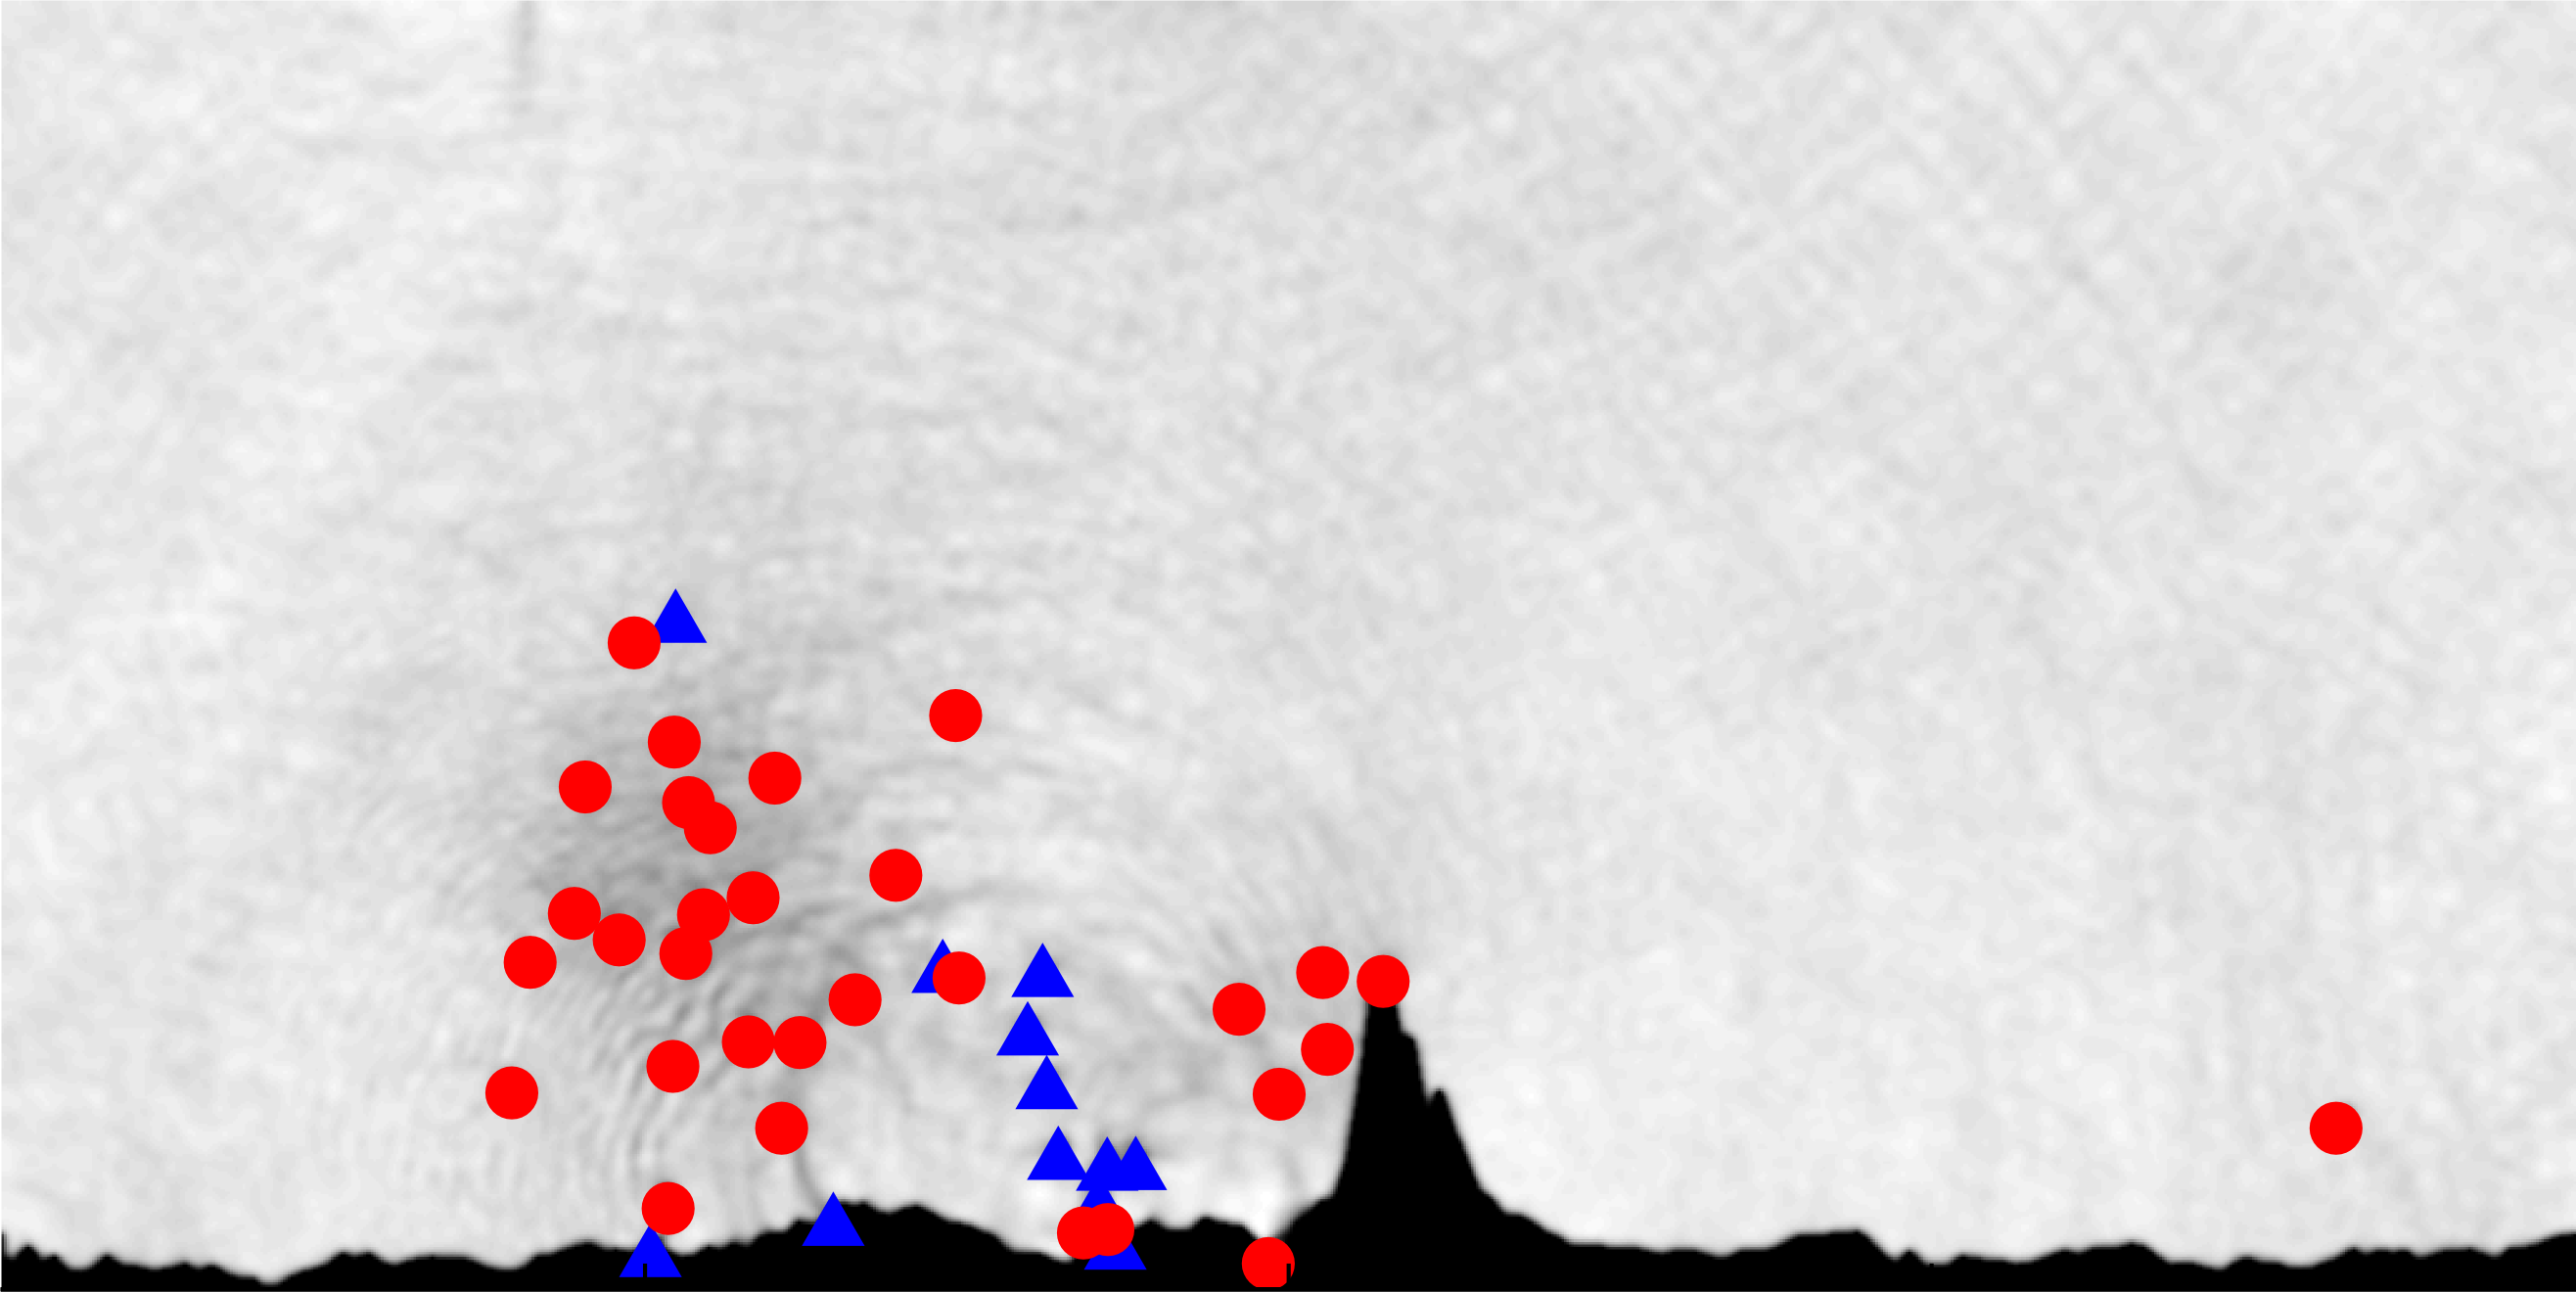
\includegraphics[width=0.35\linewidth]{./afm/figures/prog-35-1580}\hspace{-0.6cm}
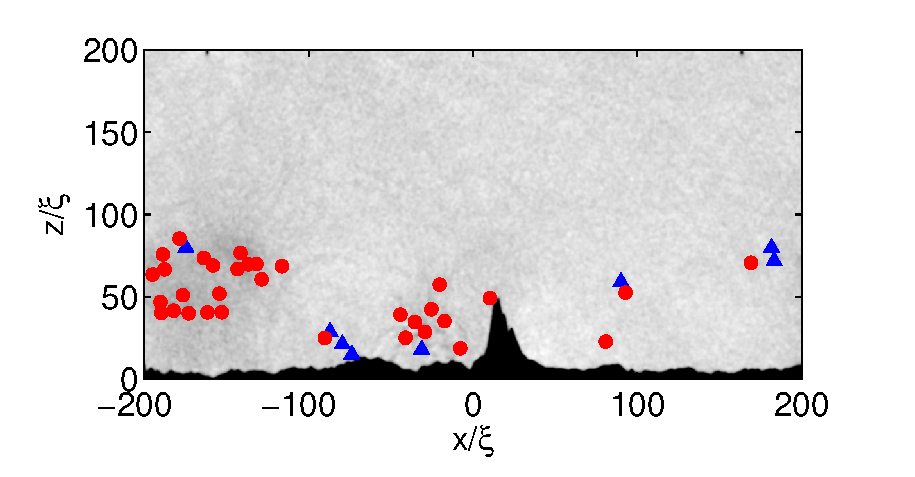
\includegraphics[width=0.35\linewidth]{./afm/figures/prog-35-2100}
\caption{\label{fig:prog} Evolution of 2D flow past the rough surface for a flow speed of $v=0.35c$.  Depicted are snapshots of density and vortex locations at times (from left to right) $t=500$, $1580$, and $2100~\tau$.  Red (blue) circles represent vortices of positive (negative) circulation.  }%Cluster forms, is interupped by secondary cluster and detaches. New cluster forms. }
\end{figure*}
\begin{figure*}
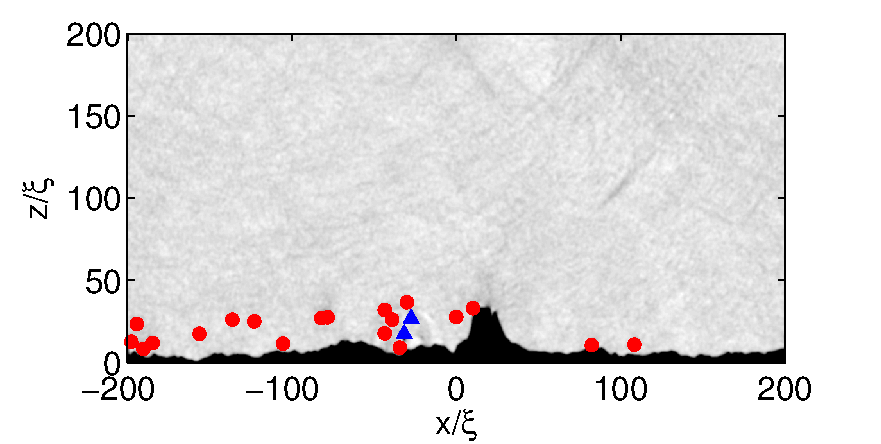
\includegraphics[width=0.35\linewidth]{./afm/figures/6th-35-2440}\hspace{-0.6cm}
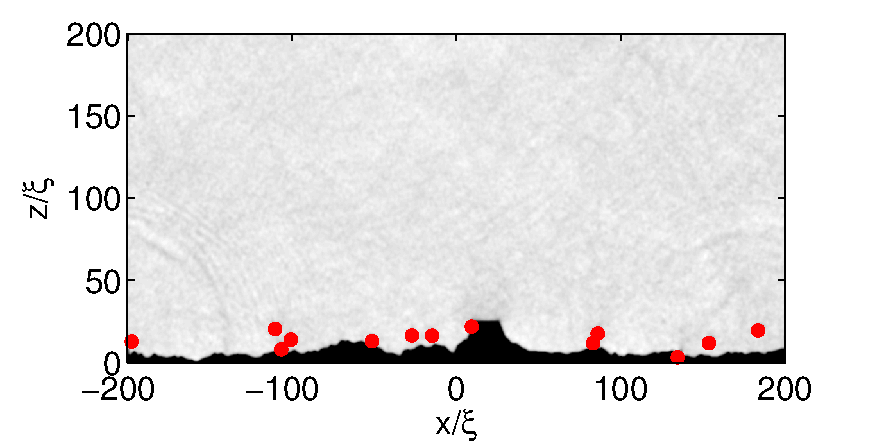
\includegraphics[width=0.35\linewidth]{./afm/figures/8th-35-2440}\hspace{-0.6cm}
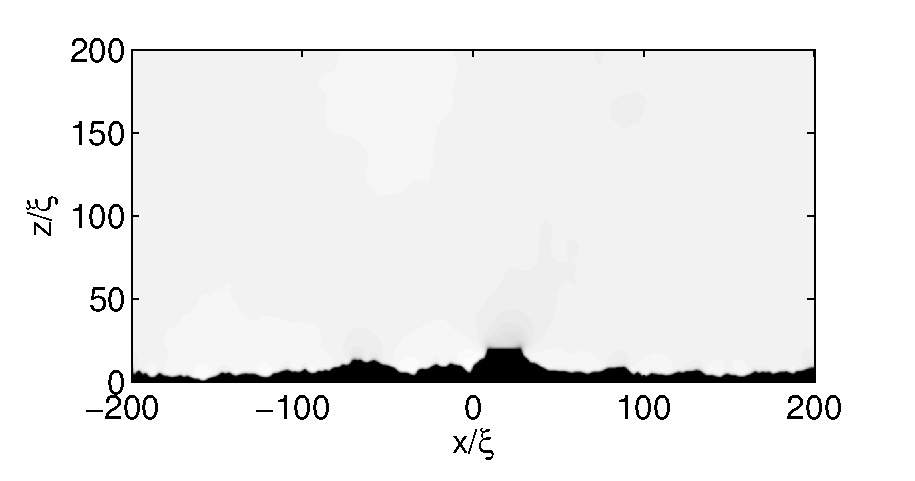
\includegraphics[width=0.35\linewidth]{./afm/figures/10th-35-2440}
\caption{\label{fig:trunc} Same-time snapshots for various levels of surface truncation: (i) $\beta=70\%$, (ii) $\beta=50\%$ and (iiii) $\beta=40\%$, where $\beta$ represents the truncation height relative to the highest point in the surface. Depicted are snapshots of density and vortex locations. For comparison, the untruncated surface ($\beta=100\%$) is depicted in Fig. \ref{fig:prog}.  The flow speed is $v=0.35c$ and the time is $t=2440\tau$.}
\end{figure*}

Superfluid flow past an obstacle at a velocity greater than a critical velocity causes 
vortices to be nucleated from the obstacle into the bulk of the fluid.  For the rough surface we consider (Fig. \ref{fig:afmimg}) the prominences acts as obstacles.  For simplicity we begin in 2D, modelling the flow past the surface depicted in Fig. \ref{fig:afmimg}(b).  We find the critical velocity for vortex nucleation to be $v_c=(0.125\pm0.025) c$.   We focus on an arbitrary super-critical flow speed of $v=0.35c$, with Fig. \ref{fig:prog} depicting the evolution of the system.  For clarity we show both the condensate density (upper plots) and vortex locations/circulation (lower plots).  At early times, a series of positive-circulation vortices (red) peel off from the peak of the large mountain. Vortices are nucleated here, and not elsewhere, due to the high curvature in the surface at this peak, which induces a relatively high local fluid velocity.  As they are carried downstream the vortices stay in close proximity and co-rotate about one another; this leads to the vortices combining into a larger-scale cluster of positive circulation.  This cluster travels downstream just above the surface.  Close to the surface, the cluster introduces a large relative fluid flow in the positive-$x$ direction.  This interrupts the nucleation of vortices from the mountain top and also induces the secondary generation of vortices (blue) from smaller-scale surface prominences.  These secondary vortices are of negative circulation and also form a vortex cluster. As this cluster grows, it leads to a cessation of secondary vortex production, and so again the primary vortices become nucleated from the mountain peak.  This process repeats.

The total number of vortices $N_v$ increases with time (Fig. \ref{fig:nvort}(a), solid line); initially this increase is rapid but over time it slows down as the number of vortices within the finite-sized box begins to saturate.  Initially this is almost entirely composed of positively-signed vortices (dashed line), apart from a small amount of spurious negative-sign vortices (dotted line).  At $t\approx 700 \tau$ the number of positive-sign vortices increases sharply; this represents the formation of secondary vortices. 

It is important to note that the generation of secondary clusters requires the surface to be rough downstream of the mountain.  If the surface is perfectly smooth downstream of the mountain, the positive-signed vortices persist.  

Note also that it is possible for tertiary vortices/clusters of positive-sign; these arise when the secondary cluster induces a sufficiently high flow speed in the negative-$x$ direction to generate vortices from the local surface roughness.

\subsection{Truncated surfaces}

It is evident above that the vortex generation is dominated by the large single prominence in the surface, with the smaller prominences having only a secondary effect.  To further analysis this we next study how the flow is affected by truncation of the surface.  Figure \ref{fig:trunc} shows a snapshot (at fixed time) for various levels of truncation $\beta$, with all cases having the same flow speed $v=0.35c$.  It is evident that the height of the mountain plays a critical role.  Already, when the mountain is capped at $70\%$, the number of vortices produced by that time is vastly reduced.  The vortices are generated at a sufficiently low frequency that only small clusters form; secondary vortices are still formed but in a much lower quantity.  For $\beta=50\%$ even fewer vortices are produced, and for this case no clustering takes place and in turn no secondary vortices are formed.  For $\beta=40\%$ no vortices are generated at all.  

\begin{figure}
\centering
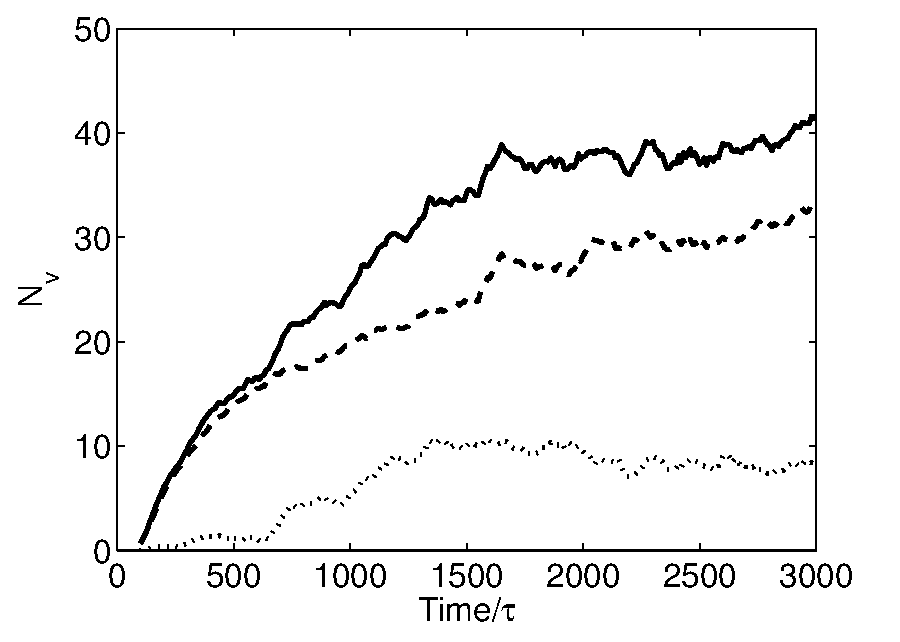
\includegraphics[width=0.45\linewidth]{./afm/figures/nvpn3bw}
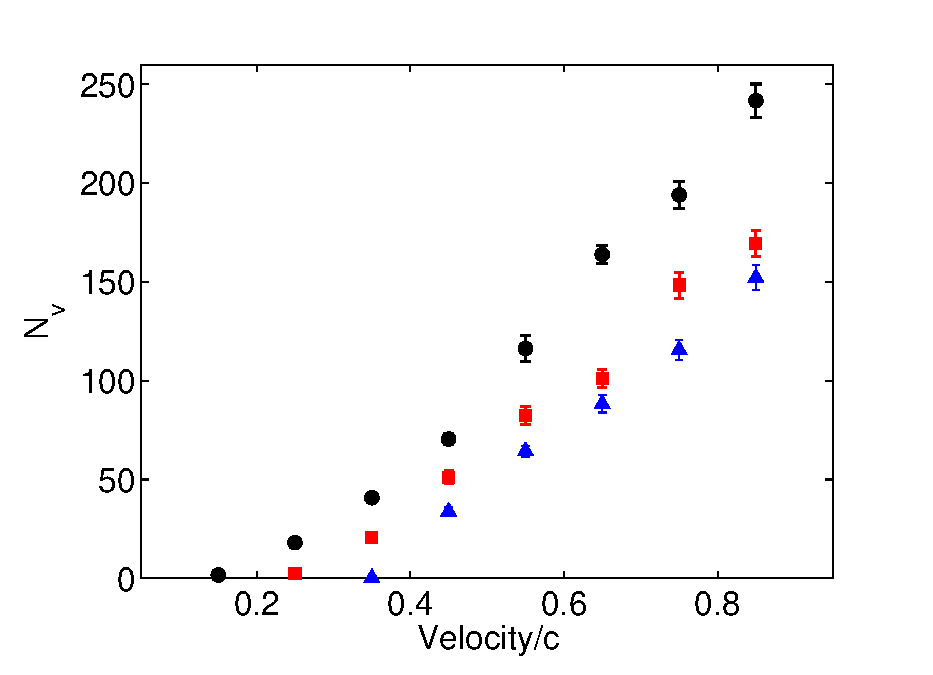
\includegraphics[width=0.45\linewidth]{./afm/figures/nv_v}
\caption{\label{fig:nvort} (a) Number of vortices produced during $v=0.35c$ flow past the surface.  Shown are the numbers of total vortices $N_v$ (solid line), positive vortices (dashed line) and negative vortices (dotted line). (b) Final number of vortices $N_v$ as a function of the flow velocity $v$ for the 2d simulations.  Each data point represents the average of 20 measurements of $N_v$ in the vicinity of $t=3000\tau$.}
\end{figure}

\subsection{Dependence on flow speed}

Figure \ref{fig:nvort}(b) shows the final number of vortices as a function of the flow speed.  For the three truncation levels considered, $N_v$ is zero up to the critical velocity and then increases in an approximately linear manner.    

\section{\label{section:3dafmlayer} 3D boundary layer and velocity statistics}
\end{chapter}
